% ==============================================================================
% Section 1.6: Case Study — Neutron
% ==============================================================================

\section{Case Study: Neutron Decay}
\label{sec:case_neutron}

\subsection{\texorpdfstring{Neutron $\beta$-Decay}{Neutron beta-Decay}: Junction Relaxation to Proton Anchor}

% --- AT-A-GLANCE BOX (KB-CANON-002) ---
\begin{edcAtAGlance}{Neutron $\beta$-Decay}
  \edcBaseline{
    Decay: $n \to p + e^- + \bar\nu_e$ with $\tau_n = 879.4 \pm 0.6$ s (PDG 2024)\\
    Q-value: $\Delta m_{np} = 1.293$ MeV available for products\\
    Mechanism: $d \to u + W^- \to u + e^- + \bar\nu_e$ (virtual $W^-$ exchange)\\
    Coupling: V$-$A structure from $SU(2)_L$ gauge theory
  }
  \edcEDCView{
    Neutron = excited Y-junction (same topology as proton, displaced from Steiner minimum)\\
    Instability: $q_n > 0$ means higher geometric energy than proton ($q=0$)\\
    Decay process: Junction relaxation $\to$ thick-brane charging $\to$ frozen projection\\
    Output: Brane modes organize into allowed channels via selection rules
  }
  \edcKeyInsight{
    The neutron is not a ``different particle'' from the proton---it is the same 5D
    Y-junction in an excited state. Decay is geometric relaxation, not a point-particle
    vertex. The ``weakness'' comes from bulk$\to$brane transfer suppression, not a
    small coupling constant.
  }
  \edcFalsifiable{
    \textbullet\ If muon channel opens without external energy ($m_\mu > Q_\beta$)\\
    \textbullet\ If energy ledger cannot close (energy ``disappears'' without accounting)\\
    \textbullet\ If mechanism predicts wrong selection rules or additional channels
  }
\end{edcAtAGlance}

\medskip

The neutron is the anchor case for the EDC weak program. Its decay provides the
clearest example of bulk$\to$brane transfer because the neutron, as a bulk-core
junction, has a component that extends into the bulk.

% ============================================================
%  THICK-BRANE SETTING
% ============================================================
\subsubsection{Thick-Brane Setting for Neutron Decay}
\label{subsec:n_thick_brane}

Before describing the neutron mechanism, we establish the thick-brane microphysical
picture that provides the physical bridge: how bulk dynamics (junction transitions)
produce observed 3D particles (electrons, neutrinos) through the mediation of a
thick brane with finite extent.

\paragraph{Thin brane vs thick brane.}
\begin{itemize}[nosep]
  \item \textbf{Thin brane:} A mathematical idealization where the 4D world-volume
        has zero thickness in the extra dimension ($\delta \to 0$). Fields are
        strictly confined to a hypersurface.
  \item \textbf{Thick brane:} A regularized model where the brane has finite
        thickness $\delta > 0$ in the extra dimension. The brane possesses two
        distinct faces:
        \begin{enumerate}[nosep]
          \item \textbf{Bulk-facing side} ($y = -\delta/2$): Interface where bulk
                fields couple to brane dynamics
          \item \textbf{Observer-facing side} ($y = +\delta/2$): Interface where
                effective 3D/4D physics emerges
        \end{enumerate}
\end{itemize}

\noindent\textbf{Why thick brane for weak processes?} The thick-brane picture provides:
\begin{enumerate}[nosep]
  \item \textbf{Regularization:} Avoids singular delta-function sources in 5D equations
  \item \textbf{Two-face structure:} Distinguishes where energy enters (bulk-facing)
        from where particles emerge (observer-facing)
  \item \textbf{Localization mechanism:} Brane-layer modes have finite transverse
        extent, enabling mode selection
  \item \textbf{Frozen boundary interpretation:} The one-way valve becomes a property
        of the observer-facing interface
\end{enumerate}

\paragraph{Core definitions/\tagP{}.}

\begin{itemize}[nosep]
  \item \textbf{Bulk-core:} The Y-junction with three flux-tube arms in the 5D bulk.
        Collective coordinate $q(t)$ parametrizes the configuration:
        $q = 0$ = proton (Steiner minimum); $q > 0$ = neutron (excited).

  \item \textbf{Brane-layer modes:} The region of finite thickness $\delta$ where
        the 4D membrane resides. Within this layer, localized field excitations
        $\phi(y, t)$ propagate, where $y \in [-\delta/2, +\delta/2]$.

  \item \textbf{Observed 3D particle states:} The effective outputs that emerge on
        the observer-facing side of the brane. These are what laboratory detectors
        register:
        \[
        \text{Brane-layer mode } \phi(y,t)
        \xrightarrow{\mathcal{P}_{\mathrm{frozen}}}
        \text{3D particle state}
        \]
\end{itemize}

\begin{tcolorbox}[edcConcept, title={Conceptual Picture: The Brane as ``Glass Window'' \tagP{}}]
\textbf{Key idea:} The brane has TWO sets of boundary conditions:
\begin{itemize}[nosep]
  \item \textbf{Left (bulk-facing):} BC toward 5D bulk (Plenum, energy fluid)
  \item \textbf{Right (observer-facing):} BC toward 3D observable universe (our physics)
\end{itemize}
Physics in 5D is the \textbf{cause}; 3D observations are the \textbf{effect}.
The thick-brane allows energy to flow from bulk structures (junctions) into
brane-localized modes, which then appear as observable particles on the 3D side.
\end{tcolorbox}

% ============================================================
%  NEUTRON AS EXCITED JUNCTION
% ============================================================
\subsubsection{What Is the Neutron in EDC Ontology?}
\label{subsec:n_ontology}

\textbf{Ontology} \tagP{}/\tagDc{}: The neutron is modeled as a \emph{bulk-core
junction} configuration whose relaxation can pump energy into the thick brane.
Unlike purely brane-dominant leptonic modes (muon, tau), the neutron carries a
``bulk-facing'' component: its decay is therefore used as the anchor case because
it naturally provides a bulk$\to$brane pumping stage.

\begin{tcolorbox}[edcCornerstone, title={Postulate: Neutron as Excited Junction \tagP{}}]
In 5D EDC, the neutron is a three-arm flux-tube junction with the \textbf{same
topological structure} as the proton, but in an \textbf{excited state}---displaced
from the Steiner minimum.

The neutron is not a ``different animal'' from the proton---it is the \textbf{same
5D object} in an excited state, destined to relax toward the Steiner minimum.
\end{tcolorbox}

\paragraph{Proton vs neutron comparison \tagDc{}.}

\begin{center}
\begin{tabular}{lcc}
\toprule
& \textbf{Proton} & \textbf{Neutron} \\
\midrule
Topology & Y-junction (3 arms) & Y-junction (3 arms) \\
Arm angles & $120\degree$ (Steiner) & $\neq 120\degree$ (excited) \\
Energy state & Ground state (minimum) & Metastable (excited) \\
Stability & Stable & Unstable ($\tau \approx 879$ s) \\
Charge (Q) & +1 & 0 \\
Collective coordinate & $q = 0$ & $q_n > 0$ \\
\bottomrule
\end{tabular}
\end{center}

\paragraph{Collective coordinate.}
Let $\hat{e}_i$ ($i = 1,2,3$) be the unit tangent vectors at the junction. The
collective coordinate measuring departure from Steiner symmetry is:
\begin{equation}
\boxed{q \equiv \frac{1}{3}\left| \hat{e}_1 + \hat{e}_2 + \hat{e}_3 \right|}
\label{eq:n_q_def}
\end{equation}

\noindent\textbf{Range and interpretation \tagDer{}:}
\begin{itemize}[nosep]
  \item $q = 0$: Steiner configuration ($\hat{e}_1 + \hat{e}_2 + \hat{e}_3 = 0$)
        $\Rightarrow$ \textbf{proton}
  \item $q = 1$: Maximal asymmetry (all arms parallel) $\Rightarrow$ unphysical limit
  \item $0 < q < 1$: Excited states, including \textbf{neutron}
\end{itemize}

Based on $\mathbb{Z}_6$ symmetry arguments, the neutron corresponds to approximately
$q_n \approx 1/3$ (half-Steiner displacement) \tagI{}.

\paragraph{Geometric excitation energy \tagDc{}.}
Any displacement from the Steiner minimum ($q = 0$) carries positive geometric energy:
\begin{equation}
E_{\text{geom}}(q) = E_0 + \kappa_q \, q^2 + O(q^4)
\label{eq:n_energy_taylor}
\end{equation}
where $\kappa_q > 0$ is the stiffness of the junction against asymmetric deformations.
Since the Steiner point is a local minimum of the total weighted length, the energy
expands as a positive-definite quadratic form to leading order.

\textbf{Corollary (instability):} The neutron ($q_n > 0$) has higher energy than the
proton ($q = 0$). This energy difference drives relaxation toward the Steiner minimum.

% --- POTENTIAL FIGURE ---
\begin{figure}[ht]
\centering
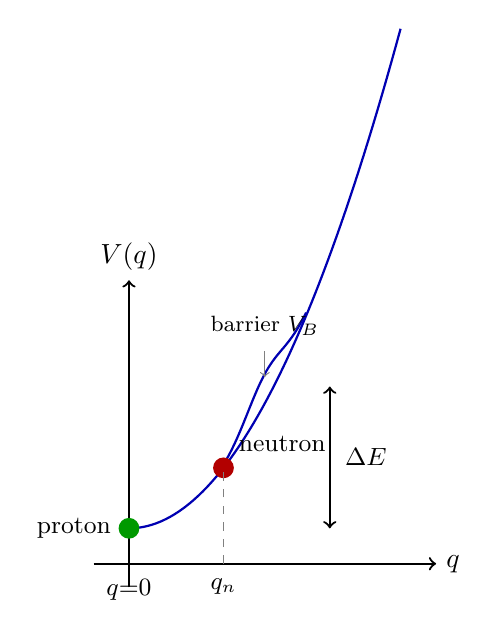
\begin{tikzpicture}[scale=1.5]
    % Axes
    \draw[thick,->] (-0.3,0) -- (2.6,0) node[right] {$q$};
    \draw[thick,->] (0,-0.2) -- (0,2.4) node[above] {$V(q)$};

    % Potential curve (base parabola)
    \draw[thick,blue!70!black,domain=0:2.3,samples=60] plot (\x, {0.3 + 0.8*\x*\x});

    % Barrier bump (schematic)
    \draw[thick,blue!70!black,domain=0.8:1.5,samples=30] plot (\x, {0.3 + 0.8*\x*\x + 0.25*exp(-18*(\x-1.15)*(\x-1.15))});

    % Proton minimum
    \fill[green!60!black] (0,0.3) circle (2.5pt);
    \node[left, xshift=-3pt, font=\small] at (0,0.3) {proton};
    \node[below, yshift=-2pt, font=\small] at (0,0) {$q{=}0$};

    % Neutron excited
    \fill[red!70!black] (0.8,0.812) circle (2.5pt);
    \node[above right, xshift=2pt, yshift=2pt, font=\small] at (0.8,0.82) {neutron};
    \draw[dashed, gray] (0.8,0) -- (0.8,0.812);
    \node[below, yshift=-2pt, font=\small] at (0.8,0) {$q_n$};

    % Energy difference arrow
    \draw[<->, thick] (1.7,0.3) -- (1.7,1.5);
    \node[right, xshift=2pt, font=\small] at (1.7,0.9) {$\Delta E$};

    % Barrier label
    \node[above, font=\footnotesize] at (1.15,1.85) {barrier $V_B$};
    \draw[->, thin, gray] (1.15,1.8) -- (1.15,1.58);
\end{tikzpicture}
\caption{\textbf{Schematic potential $V(q)$ for the junction coordinate.} The proton
sits at $q=0$ (Steiner minimum); the neutron at $q_n > 0$ (metastable excited state).
A barrier $V_B$ separates neutron from proton, determining the tunneling lifetime.}
\label{fig:n_potential}
\end{figure}

\paragraph{Baseline observable \tagBL{}.}
Experimentally, the dominant channel is:
\begin{equation}
n \to p + e^- + \bar\nu_e,
\label{eq:n_channel}
\end{equation}
with a Q-value governed by the neutron--proton mass difference:
$\Delta m_{np} = m_n - m_p \approx 1.293$ MeV \tagBL{}.

EDC does not dispute the baseline; it supplies an interface mechanism that makes
the channel structure intelligible.

% ============================================================
%  MECHANICS PICTURE
% ============================================================
\subsubsection{Mechanics Picture: Ring + 3 Springs}
\label{subsec:n_mechanics}

To build intuition for the junction dynamics, we introduce a mechanical analogy.

\begin{tcolorbox}[edcModel, title={Mechanical Analogy: Ring + 3 Springs \tagI{}/\tagP{}}]
Consider a circular ring of radius $R$ with three springs attached at angles
$\theta_1, \theta_2, \theta_3$, each pulling toward the center with spring
constant $k$. The springs represent flux-tube tensions; the ring represents a
collective constraint.

\medskip
\textbf{Interpretation:}
\begin{itemize}[nosep]
  \item Equilibrium: $\theta_1 = \theta_2 = \theta_3 = 120\degree$ (proton)
  \item Excited: angles deviate, springs store extra energy (neutron)
  \item Ring constraint couples all three modes (collective dynamics)
\end{itemize}
\end{tcolorbox}

\paragraph{Three-mode decomposition.}
The junction has three angular degrees of freedom $(\theta_1, \theta_2, \theta_3)$
subject to $\theta_1 + \theta_2 + \theta_3 = 2\pi$. This leaves two independent modes:
\begin{align}
q &= \text{(collective asymmetry)} = \frac{1}{3}|\hat{e}_1 + \hat{e}_2 + \hat{e}_3|
    \tag{radial} \\
\perp_1, \perp_2 &= \text{(transverse modes)} \tag{angular}
\end{align}
The collective coordinate $q$ measures overall departure from Steiner; the
transverse modes $\perp_{1,2}$ describe shape distortions at fixed $q$.

For slow (adiabatic) relaxation, the transverse modes equilibrate quickly, and
the effective dynamics is one-dimensional in $q$. This justifies the 1D WKB
treatment \tagI{}.

\paragraph{Linearized oscillation.}
Near the metastable neutron configuration $q = q_n$, the dynamics linearizes to:
\begin{equation}
\ddot{q} + 2\gamma \dot{q} + \omega_0^2 (q - q_n) = 0
\label{eq:n_damped_oscillator}
\end{equation}
where $\omega_0$ = natural frequency (junction stiffness) \tagP{}, and
$\gamma$ = effective damping (energy loss to brane modes) (open).

\textbf{Note:} This is a \textbf{mechanical linearization} around a geometric
minimum---not a quantum field theory oscillator. It captures the qualitative
behavior: the junction oscillates around its metastable position while losing
energy to the brane.

% ============================================================
%  PHYSICAL PROCESS NARRATIVE
% ============================================================
\subsubsection{The Mechanistic Story: The ``Film'' of Neutron Decay}
\label{subsec:n_film}

We narrate the process following the canonical \textbf{Physical Process Narrative
(PPN)} framework for energy transfer in EDC.

\begin{tcolorbox}[edcPPN, title={Physical Process Narrative (PPN): Bulk $\to$ Brane $\to$ Observer}]
\begin{enumerate}[nosep,leftmargin=*]
  \item[\textbf{(i)}] \textbf{Bulk cause (5D):} Change in bulk-core configuration
        $q(t)$ (junction displacement from Steiner) releases geometric energy
        $\Delta E \approx \Delta m_{np}c^2$.

  \item[\textbf{(ii)}] \textbf{Injection to brane:} This change pumps energy into
        brane-layer modes $\phi$ at the bulk-facing boundary via
        $\mathcal{L}_{\mathrm{int}} = g\,q(t)\,\phi(-\delta/2,t)$.

  \item[\textbf{(iii)}] \textbf{Absorption:} The brane accepts the excess energy
        from the bulk process and stores it as excitations of its degrees of
        freedom (brane-layer storage).

  \item[\textbf{(iv)}] \textbf{Dissipation/relaxation:} Within the brane-layer,
        energy redistributes across modes, loses coherence (coarse-graining/decoherence),
        and flows toward allowed output channels.

  \item[\textbf{(v)}] \textbf{Frozen projection (observer side):} The operator
        $\mathcal{P}_{\mathrm{frozen}}$ maps brane-layer excitations to observable
        3D outputs ($e^- + \bar{\nu}_e + \text{recoil}$), enforcing selection rules.

  \item[\textbf{(vi)}] \textbf{Ledger closure:} Total 5D conservation holds; the
        brane redirects energy/quantum numbers from bulk channels to observer
        channels without ``magical disappearance.''
\end{enumerate}
\end{tcolorbox}

\paragraph{Stage A: Absorption (brane charging by junction relaxation).}

A junction relaxation in the bulk-core sector induces a bulk-facing pumping into
the brane layer. In the effective brane coordinate picture, we model this as a
trajectory $q(t)$ in an effective potential $V(q)$, with instantaneous pumping
power:
\begin{equation}
\Pi_{\text{pump}}(t) \equiv -\dot{q}(t) \cdot \partial_q V(q(t)).
\label{eq:n_pump}
\end{equation}

\textbf{Interpretation} \tagDc{}: The quantity $\Pi_{\text{pump}}$ is not a new
force; it is the power delivered into the brane reservoir by the bulk-side
relaxation mechanism. When $\dot{q} < 0$ (relaxation toward $q=0$) and
$\partial_q V > 0$ (uphill from neutron side), the product is positive.

The accumulated energy delivered into the brane up to time $t$ is the charging
integral:
\begin{equation}
E_{\text{charge}}(t) \equiv \int_0^t \Pi_{\text{pump}}(t')\,dt'.
\label{eq:n_charge}
\end{equation}

\paragraph{Stage B: Dissipation (redistribution into brane-layer modes) \tagP{}.}

Once energy is deposited, it need not be immediately released. A thick brane
provides internal degrees of freedom (layer modes) into which the reservoir
energy can redistribute:
\begin{equation}
E_{\text{brane}} \;\to\; \{\phi_k\}_{\text{layer modes}}.
\label{eq:n_modes}
\end{equation}

This stage is crucial: without it, one cannot explain why the observed outputs
appear as a restricted set rather than an arbitrary energy dump.

The coupling of the junction coordinate $q(t)$ to brane-layer modes induces an
effective dissipation. Integrating out the fast brane degrees of freedom yields
a damped equation of motion \tagP{}:
\begin{equation}
\boxed{M \ddot{q} + \Gamma \dot{q} + \partial_q V(q) = 0}
\label{eq:n_damped_motion}
\end{equation}
where $M$ = effective mass (junction inertia), $\Gamma$ = effective damping
coefficient (brane-layer dissipation), and $V(q)$ = effective potential from
junction geometry (Fig.~\ref{fig:n_potential}).

\textbf{Physical interpretation of $\Gamma$} \tagP{}: The coefficient
$\Gamma$ encodes the energy transfer rate from the bulk-core junction to brane-layer
modes. $\Gamma = 0$ means no coupling (unphysical); $\Gamma > 0$ means junction
energy drains into brane modes. Note: $\Gamma$ is NOT fitted to the neutron
lifetime $\tau_n$ in this chapter. Its derivation from thick-brane microphysics
remains (open).

\paragraph{Stage C: Release (observer-facing projection into 3D outputs) \tagDc{}.}

The release stage begins when the system enters a regime where pumping becomes
negligible compared to release:
\begin{equation}
\Xi(t) \equiv \frac{\Pi_{\text{pump}}(t)}{\Pi_{\text{release}}(t)} \ll 1
\quad\text{at } t = t_*.
\label{eq:n_trigger}
\end{equation}

\textbf{Important nuance}: We do not claim that $\dot{q}(t_*) = 0$ exactly.
Rather, the interface becomes \emph{effectively frozen} at observational
resolution: the continuous pump term is negligible, and the release can be
treated as the dominant process.

The observer-facing outputs are defined by the frozen projection operator
:
\begin{equation}
\{\text{outputs}\}_{3D} = \mathcal{P}_{\text{frozen}}\big(\{\phi_k\}\big),
\qquad
\mathcal{P}_{\text{frozen}} = \mathcal{P}_{\text{energy}} \circ
\mathcal{P}_{\text{mode}} \circ \mathcal{P}_{\text{chir}}.
\label{eq:n_projection}
\end{equation}

% ============================================================
%  CANONICAL GLOSSARY BOX
% ============================================================
\begin{tcolorbox}[edcCanonical, title={Canonical Brane-Language for Neutron Decay}]
The neutron decay process involves \textbf{three conceptually distinct phases},
all part of a single energy-conserving flow:

\medskip
\textbf{(1) Absorption / Charging} (bulk $\to$ brane-layer) \tagDc{}\\
The brane \textbf{receives} energy from the relaxing bulk-core junction. This is
not ``creation''---it is \emph{transfer} governed by the coupling $\mathcal{L}_{\mathrm{int}}$.

\emph{Ledger:} $\Delta E_{\mathrm{brane}} = -\Delta E_{\mathrm{bulk}} - E_{\mathrm{other}}$

\medskip
\textbf{(2) Dissipation / Redistribution} (within brane-layer) \tagP{}\\
Internal brane-layer dynamics \textbf{redistribute} the absorbed energy into allowed
mode excitations $\{\phi_k\}$. ``Dissipation'' does \textbf{not} mean energy loss---it
means transition from coherent pumping channel to spectral mode distribution.

\emph{Mechanism:} Characterized by $\Gamma_{\mathrm{eff}}$ (effective redistribution rate).

\medskip
\textbf{(3) Release / Emission} (brane-layer $\to$ 3D observer) \tagDc{}/\tagP{}\\
The frozen projection operator $\mathcal{P}_{\mathrm{frozen}}$ \textbf{maps} brane-layer
modes to allowed 3D particle outputs. This is \emph{not} ``particle creation from
nothing''---it is a boundary projection enforcing selection rules.

\emph{Output:} $\{\phi_k\} \xrightarrow{\mathcal{P}_{\mathrm{frozen}}}
\{e^-, \bar{\nu}_e, \mathrm{recoil}, \mathrm{soft}\}_{\mathrm{3D}}$

\medskip
\hrule
\medskip
\textbf{One-liner (citable):}
\begin{quote}
\emph{``Neutron decay in EDC is bulk-core relaxation that charges the brane
(absorption), the brane redistributes energy into layer modes (dissipation),
and the observer-facing boundary projects those modes into allowed 3D particle
outputs (release).''}
\end{quote}
\end{tcolorbox}

% ============================================================
%  FROZEN PROJECTION MECHANISM
% ============================================================
\subsubsection{Frozen Projection Boundary}
\label{subsec:n_frozen}

\paragraph{One-way valve mechanism \tagDc{}/\tagP{}.}
The frozen projection boundary acts as a \textbf{one-way valve}:
\begin{itemize}[nosep]
  \item \textbf{INFLOW} (bulk $\to$ brane): spontaneously allowed
  \item \textbf{OUTFLOW} (brane $\to$ bulk): energetically/kinematically suppressed
\end{itemize}

\textbf{Physical interpretation:} The boundary condition at the observer-facing
side ``freezes'' high-energy bulk modes, preventing their re-excitation from the
3D side. This is analogous to decoherence: environmental tracing eliminates
coherent bulk superpositions.

\paragraph{Formal definition/\tagDc{}.}
Let $\phi(y, t)$ denote the brane-layer field, where $y \in [-\delta/2, +\delta/2]$
is the coordinate across the brane thickness. The \textbf{frozen projection operator}
$\mathcal{P}_{\mathrm{frozen}}$ maps brane-layer excitations at the observer-facing
boundary to observable 3D particle states:
\begin{equation}
\boxed{\mathcal{P}_{\mathrm{frozen}}: \quad
\phi\bigl(y = +\tfrac{\delta}{2}, t\bigr) \;\longmapsto\;
\{e^-, e^+, \nu_e, \bar{\nu}_e, \gamma, \ldots\}_{\mathrm{3D}}}
\label{eq:n_frozen_projection}
\end{equation}

The operator acts as follows:
\begin{enumerate}[nosep]
  \item Identifies modes satisfying the frozen criterion ($\hbar\omega \gg E_{\mathrm{env}}$)
  \item Projects these onto mass-shell particle states
  \item Enforces selection rules (charge, lepton number, energy threshold)
\end{enumerate}

\paragraph{Frozen criterion/\tagDc{}.}
A brane-layer mode with characteristic frequency $\omega$ is \textbf{frozen}
(appears as a fixed particle rather than a fluctuating field) when:
\begin{equation}
\boxed{\hbar\omega \gg E_{\mathrm{env}}}
\label{eq:n_frozen_criterion}
\end{equation}
where $E_{\mathrm{env}}$ is the typical environmental energy scale on the 3D side.
For neutron decay at room temperature ($E_{\mathrm{env}} \sim k_B T \sim 0.025$ eV),
all decay products ($e^-$, $\bar{\nu}_e$ with energies $\sim$ keV--MeV) satisfy
$\hbar\omega \gg E_{\mathrm{env}}$ and thus appear as stable particles.

\paragraph{Irreversibility \tagDc{}/\tagP{}.}
The frozen projection is effectively \textbf{irreversible}: once energy passes
through $\mathcal{P}_{\mathrm{frozen}}$ and materializes as 3D particles, it
cannot spontaneously return to bulk-core excitations. This explains why neutron
decay is observed but ``inverse beta decay'' ($p + e^- + \bar{\nu}_e \to n$)
requires external energy input.

% ============================================================
%  SELECTION RULES
% ============================================================
\subsubsection{Why the Electron Channel Is Allowed but the Muon Channel Is Not}
\label{subsec:n_selection}

A common confusion is to phrase this as ``EDC forbids the muon channel.'' The
correct, book-level statement is purely kinematic and belongs to
$\mathcal{P}_{\text{energy}}$.

\paragraph{Baseline kinematic gate \tagBL{}.}
For $\beta$-decay, the available energy budget is set by:
\begin{equation}
Q_\beta(\ell) \approx \Delta m_{np} - m_\ell - m_\nu \approx \Delta m_{np} - m_\ell,
\label{eq:n_Q_beta}
\end{equation}
where neutrino masses are negligible at this scale.

\paragraph{Electron channel.}
For $\ell = e$ one has $m_e \approx 0.511$ MeV \tagBL{}, hence $Q_\beta(e) > 0$,
so phase space exists and the channel is kinematically open:
\begin{equation}
Q_\beta(e) \approx 1.293 - 0.511 = 0.782~\text{MeV} > 0.
\label{eq:n_Qbeta_electron}
\end{equation}

\paragraph{Muon channel.}
For $\ell = \mu$ one has $m_\mu \approx 105.7$ MeV \tagBL{}, hence
$Q_\beta(\mu) < 0$:
\begin{equation}
Q_\beta(\mu) \approx 1.293 - 105.7 \approx -104.4~\text{MeV} < 0,
\label{eq:n_Qbeta_muon}
\end{equation}
meaning there is \emph{no kinematically allowed phase space} for
$n \to p + \mu^- + \bar\nu_\mu$ at rest.

\begin{tcolorbox}[edcGuardrail, title={Q-Gate Selection Rule}]
The ``muon channel'' is rejected not by metaphysical prohibition, but because
$\mathcal{P}_{\text{energy}}$ yields zero support:
\begin{equation}
\mathcal{P}_{\text{energy}}: \quad
\text{channel allowed} \iff Q_\beta(\ell) > 0.
\label{eq:n_Penergy_gate}
\end{equation}
This is a kinematic fact \tagBL{}, not an EDC-specific assumption.
\end{tcolorbox}

\paragraph{What ``forbids'' means physically.}
The word ``forbids'' is not metaphysical; it has a precise kinematic meaning:

\begin{itemize}[nosep]
  \item \textbf{Energy budget}: The neutron at rest has total energy $m_n c^2$.
        After decay, the products must share this energy (minus binding).
  \item \textbf{Rest mass floor}: The \emph{minimum} energy required to produce
        $p + \mu^- + \bar\nu_\mu$ is their combined rest masses:
        $m_p + m_\mu + m_\nu \approx 938.3 + 105.7 + 0 = 1044$ MeV.
  \item \textbf{Comparison}: But $m_n c^2 \approx 939.6$ MeV $<$ 1044 MeV.
  \item \textbf{Conclusion}: There is \emph{no real final state} satisfying
        energy-momentum conservation. The muon channel is kinematically closed.
\end{itemize}

\noindent
A muon \emph{can} appear as a \textbf{virtual particle} in loop diagrams (off-shell),
but it cannot emerge as a real, on-shell particle in the final state without an
external energy source. This is standard relativistic kinematics \tagBL{}, not an
EDC claim.

\paragraph{EDC interpretation.}
This is exactly what we want from the pipeline language: one can separate
\emph{what is purely kinematic} (baseline gating) from \emph{what is mechanistic}
(how the brane actually processes and projects the allowed energy into specific
outputs). In neutron decay, $\mathcal{P}_{\text{energy}}$ restricts us to the
electron sector; the remaining question is then: \emph{given that the electron
channel is open, what interface mechanism produces the observed
$\{e^-, \bar\nu\}$ outputs?}

\paragraph{Selection rules summary \tagDc{}.}
The frozen boundary imposes selection rules on which decay products can emerge:
\begin{enumerate}[nosep]
  \item \textbf{Charge conservation:} $Q_{\text{in}} = Q_{\text{out}}$
        (neutron: $0 \to +1 + (-1) + 0$)
  \item \textbf{Lepton number:} $L_e: 0 \to 0 + 1 + (-1) = 0$ (\checkmark)
  \item \textbf{Energy threshold:} $\Delta E > m_e c^2$ required for electron emission
  \item \textbf{Momentum matching:} recoil absorbed by proton
\end{enumerate}

\textbf{Suppressed channels:}
\begin{itemize}[nosep]
  \item $n \to p + \mu^- + \bar{\nu}_\mu$: Forbidden by $m_\mu > \Delta E$
  \item $n \to p + \gamma$: Suppressed (no photon channel in lowest-order weak)
  \item $n \to p + e^- + e^+ + \nu_e + \bar{\nu}_e$: Phase space suppressed
\end{itemize}

\paragraph{V--A structure \tagBL{}.}
The $V-A$ (vector minus axial-vector) structure of weak interactions is
\textbf{not derived here}---it is input from Standard Model phenomenology.
EDC provides the energy release mechanism; the detailed interaction vertex is
inherited.

% ============================================================
%  ENERGY BOOKKEEPING
% ============================================================
\subsubsection{Ledger Closure for Neutron Decay}
\label{subsec:n_ledger}

The neutron case forces discipline on bookkeeping. The brane reservoir must close
its ledger: the energy deposited by junction relaxation must appear as observable
kinetic energies plus any additional channels consistent with conservation.

\paragraph{Charging ledger \tagDc{}.}
During the charging phase, energy conservation requires:
\begin{equation}
\boxed{\Delta E_{\mathrm{brane}} = -\Delta E_{\mathrm{bulk}} - E_{\mathrm{other}}}
\label{eq:n_charging_ledger}
\end{equation}
where:
\begin{itemize}[nosep]
  \item $\Delta E_{\mathrm{bulk}} = E(q{=}0) - E(q{=}q_n) < 0$ (bulk loses geometric
        excitation energy)
  \item $\Delta E_{\mathrm{brane}} > 0$ (brane gains stored energy)
\end{itemize}

The residual term $E_{\mathrm{other}}$ decomposes as:
\begin{equation}
E_{\mathrm{other}} = E_{\mathrm{recoil}} + E_{\mathrm{soft}} + E_{\mathrm{bulk\,residual}}
\label{eq:n_e_other}
\end{equation}
\begin{itemize}[nosep]
  \item $E_{\mathrm{recoil}}$: 3D momentum balance (proton recoil) \tagDc{}
  \item $E_{\mathrm{soft}}$: low-energy brane modes, soft photons/phonons \tagP{}
  \item $E_{\mathrm{bulk\,residual}}$: any energy remaining in bulk (if leakage
        permitted) \tagP{}
\end{itemize}

\paragraph{Schematic ledger identity/\tagDc{}.}
\begin{equation}
\Delta E_{\text{available}} = K_p + K_e + K_{\bar\nu} + E_{\text{other}},
\label{eq:n_ledger}
\end{equation}
where:
\begin{itemize}[nosep]
  \item $\Delta E_{\text{available}}$ is the energy budget ($\sim Q_\beta$),
  \item $K_p, K_e, K_{\bar\nu}$ are the kinetic energies of the outputs,
  \item $E_{\text{other}} = E_{\text{recoil}} + E_{\text{soft}} + E_{\text{bulk,res}}$
        collects subleading channels/(open).
\end{itemize}

For neutron decay: $|\Delta E_{\mathrm{bulk}}| \approx \Delta m_{np} c^2 \approx
1.293$ MeV \tagBL{} (PDG neutron--proton mass difference).

% --- ENERGY BOOKKEEPING TABLE ---
\begin{table}[ht]
\centering
\caption{Energy Bookkeeping for Neutron $\beta^-$ Decay \tagDc{}/\tagP{}}
\label{tab:n_energy_bookkeeping}
\small
\begin{tabular}{@{}lllll@{}}
\toprule
\textbf{Term} & \textbf{Meaning} & \textbf{Tag} & \textbf{Units} & \textbf{Location} \\
\midrule
$\Delta E_{\mathrm{bulk}}$ & Junction relaxation energy & \tagDc{} & MeV & Bulk-core \\
$\Delta E_{\mathrm{brane}}$ & Stored brane energy (charging) & \tagDc{} & MeV & Brane-layer \\
$E_e$ & Electron kinetic + rest mass & \tagBL{} & MeV & 3D output \\
$E_{\bar{\nu}}$ & Antineutrino energy & \tagBL{} & MeV & 3D output \\
$E_{\mathrm{recoil}}$ & Proton recoil & \tagDc{} & keV & 3D output \\
$E_{\mathrm{soft}}$ & Soft photons/phonons & \tagP{} & $\ll$ keV & Brane/3D \\
$E_{\mathrm{bulk\,res.}}$ & Bulk residual (if any) & \tagP{} & --- & Bulk \\
\midrule
\multicolumn{5}{@{}l@{}}{\textbf{Conservation check:} $|\Delta E_{\mathrm{bulk}}|
= \Delta E_{\mathrm{brane}} + E_{\mathrm{other}}$} \\
\multicolumn{5}{@{}l@{}}{\textbf{Release check:} $\Delta E_{\mathrm{brane}}
= E_e + E_{\bar{\nu}} + E_{\mathrm{recoil}} + E_{\mathrm{soft}}$} \\
\midrule
\multicolumn{5}{@{}l@{}}{\textbf{Numerical benchmark} \tagBL{}:
$|\Delta E_{\mathrm{bulk}}| \approx 1.293$ MeV (PDG)} \\
\bottomrule
\end{tabular}
\end{table}

% ============================================================
%  PROCESS DIAGRAM
% ============================================================
\subsubsection{Process Diagram: Neutron Decay}
\label{subsec:n_diagram}

\begin{center}
\begin{tikzpicture}[
  scale=0.85,
  box/.style={rectangle, rounded corners=4pt, minimum width=2cm, minimum height=0.8cm,
              draw=black, thick, font=\footnotesize, align=center},
  gate/.style={rectangle, rounded corners=2pt, minimum width=1.5cm, minimum height=0.6cm,
               draw=red!60!black, thick, fill=red!10, font=\scriptsize, align=center},
  arrow/.style={-{Stealth[length=5pt]}, thick},
  label/.style={font=\scriptsize\itshape, text=gray!60!black}
]

% Stage boxes
\node[box, fill=gray!20] (junction) at (0,0) {Junction\\relaxation};
\node[box, fill=red!15] (pump) at (3,0) {$\Pi_{\text{pump}}$\\absorption};
\node[box, fill=yellow!20] (modes) at (6,0) {$\{\phi_k\}$\\dissipation};
\node[box, fill=green!15] (project) at (9,0) {$\mathcal{P}_{\text{frozen}}$\\release};

% Q-gate
\node[gate] (qgate) at (6,-1.8) {Q-gate\\$Q_\beta(e)>0$\\$Q_\beta(\mu)<0$};

% Outputs
\node[box, fill=blue!15] (p) at (12,0.8) {$p$};
\node[box, fill=blue!15] (e) at (12,0) {$e^-$};
\node[box, fill=blue!15] (nu) at (12,-0.8) {$\bar\nu_e$};

% Arrows
\draw[arrow] (junction) -- (pump);
\draw[arrow] (pump) -- (modes);
\draw[arrow] (modes) -- (project);
\draw[arrow] (project) -- (p);
\draw[arrow] (project) -- (e);
\draw[arrow] (project) -- (nu);
\draw[arrow, dashed, red!50] (modes) -- (qgate);
\draw[arrow, dashed, red!50] (qgate) -- (project);

% Labels
\node[label, above] at (1.5,0.3) {bulk$\to$brane};
\node[label, above] at (4.5,0.3) {redistribute};
\node[label, above] at (7.5,0.3) {filter};
\node[label, above] at (10.5,0.5) {project};

% Ledger box
\node[rectangle, draw=gray, rounded corners=3pt, fill=gray!5,
      font=\scriptsize, align=left, text width=2.5cm] at (14.5,0)
  {Ledger:\\$\Delta E = K_p + K_e$\\$\phantom{\Delta E =} + K_{\bar\nu} + E_{\text{other}}$};

\end{tikzpicture}
\end{center}

\paragraph{Decay process mapping \tagDc{}.}

\begin{center}
\begin{tabular}{p{4cm}cp{5cm}}
\toprule
\textbf{5D (Cause)} & & \textbf{3D (Effect)} \\
\midrule
Junction relaxes: $q_n \to 0$ & $\Rightarrow$ & $n \to p$ \\
Energy pumped to brane: $\Delta E \approx 1.293$ MeV & $\Rightarrow$ & Kinetic energy of products \\
Brane modes organize via selection rules & $\Rightarrow$ & $e^- + \bar{\nu}_e$ emission \\
\bottomrule
\end{tabular}
\end{center}

% ============================================================
%  OBSERVABLE BENCHMARKS
% ============================================================
\subsubsection{Observable Benchmarks (No Fitting)}
\label{subsec:n_benchmarks}

This section lists observable quantities and their status in the EDC neutron model.
\textbf{No parameters are fitted in this case study.}

\begin{center}
\begin{tabular}{lccl}
\toprule
\textbf{Observable} & \textbf{Value} & \textbf{Status} & \textbf{Notes} \\
\midrule
Neutron lifetime $\tau_n$ & $879.4 \pm 0.6$ s & \tagBL{} & PDG 2024 \\
Mass difference $\Delta m_{np}$ & 1.293 MeV & \tagBL{} & CODATA \\
$Q$-value ($n \to p + e + \bar{\nu}$) & 0.782 MeV & \tagBL{} & Kinematic endpoint \\
Proton recoil & $\sim$ keV & \tagBL{} & Small due to mass ratio \\
\midrule
$\Delta m_{np}$ from $\mathbb{Z}_6$ breaking & 1.30 MeV & \tagDc{} & From geometry \\
$q_n \approx 1/3$ & identified & \tagI{} & Half-Steiner (OPR-24) \\
Barrier height $V_B$ & $\sim 2.6$ MeV & \tagCal{} & Fitted to $\tau_n$ (OPR-23) \\
\bottomrule
\end{tabular}
\end{center}

\textbf{Important \tagCal{}:} The neutron lifetime $\tau_n \approx 879$ s can be
reproduced via WKB tunneling through a barrier $V_B$. However, $V_B$ is
\textbf{calibrated} to match $\tau_n$, not derived from first principles. A
first-principles derivation of $V_B$ (or equivalently, the attempt frequency
$\Gamma_0$) remains (open).

% ============================================================
%  OPEN PROBLEMS
% ============================================================
\subsubsection{Open Problems for the Neutron Case}
\label{subsec:n_open}

\begin{enumerate}[nosep]
  \item \textbf{Derive $V_B$ from 5D action} (open) (OPR-23): Current status is $V_B
        \approx 2.6$ MeV (calibrated). Goal: show $V_B$ emerges from junction
        geometry + brane tension. Would upgrade $\tau_n$ from \tagCal{} to \tagDer{}.

  \item \textbf{WKB--Damping Bridge} (open): The WKB treatment uses tunneling
        through $V(q)$; this section uses damped oscillator + pumping. Goal: show
        equivalence in appropriate limits.

  \item \textbf{Thick-brane coupling $g$} (open): Postulated in
        $\mathcal{L}_{\mathrm{int}} = g\,q(t)\,\phi$. Need: derive from 5D action
        or constrain from observables.

  \item \textbf{Precise value of $q_n$} \tagI{} (OPR-24): Currently $q_n \approx
        1/3$ from $\mathbb{Z}_6$ symmetry arguments. Need: reconcile or derive from
        first principles.
\end{enumerate}

% ============================================================
%  FALSIFIABILITY HOOKS
% ============================================================
\subsubsection{Falsifiability Hooks}
\label{subsec:n_falsifiability}

\begin{tcolorbox}[falsifiability]
The neutron mechanistic story can be wrong. The most direct falsifiability hooks are:
\begin{itemize}[nosep]
  \item If the mechanism predicts additional leading-order outputs beyond
        $\{p, e^-, \bar\nu_e\}$ in the neutron Q-window, it fails.
  \item If $\mathcal{P}_{\text{energy}}$ gating is not respected (i.e., if the
        model leaks into the $\mu$ channel without external energy), it fails.
  \item If the ledger cannot be closed without hidden tuning (i.e., energy
        ``disappears'' without accounted bins), it fails.
  \item If the trigger condition requires an ad hoc fitted parameter rather
        than a regime statement, it fails.
  \item If $E_{\mathrm{other}}$ lacks structure (e.g., all energy goes to
        $e^- + \bar{\nu}$ with no recoil accounting), the ledger picture must
        be revised.
  \item If the frozen projection cannot exclude forbidden channels (e.g.,
        $\gamma + p$, $\mu^- + \bar{\nu}_\mu + p$), the weak-sector narrative fails.
\end{itemize}
\end{tcolorbox}

\begin{tcolorbox}[edcGuardrail, title={Epistemic Guardrail: Observation vs.\ Explanation}]
\textbf{(1) Baseline observable} \tagBL{}:\\
The neutron lifetime $\tau_n = 878.4 \pm 0.5\,\mathrm{s}$ is an \textbf{empirical
fact} measured in 3D. It is \textbf{not} a parameter we choose or fit in this chapter.

\medskip
\textbf{$\tau_n$ is not a control knob:} We treat $\tau_n$ as a \textbf{benchmark}
\tagBL{}, not as a tuning target. Any mapping $\tau_n \leftrightarrow
(\Gamma, g, \delta, \ldots)$ is deferred to (open) work.

\medskip
\textbf{(2) Theoretical explanation} \tagP{}/\tagDc{}:\\
The EDC claim is that $\tau_n$ is \textbf{explained} (not tuned) by the bulk-to-brane
relaxation mechanism.

\medskip
\textbf{(3) Placeholder parameters} (open):\\
Any effective parameters introduced ($\Gamma$, $g$, $\delta$, $\Pi_{\mathrm{pump}}$,
etc.) are \textbf{microphysical placeholders} until derived from the brane model.
\end{tcolorbox}

% ==============================================================================
% STOPLIGHT VERDICT (2026-01-29)
% ==============================================================================
\subsubsection{Stoplight Verdict}
\label{subsec:neutron_stoplight}

\begin{tcolorbox}[colback=yellow!10!white, colframe=orange!60!black,
    title=\textbf{Case Neutron: Stoplight Verdict}]

\begin{center}
\begin{tabular}{@{}lll@{}}
\toprule
\textbf{Claim} & \textbf{Status} & \textbf{Tag} \\
\midrule
Bulk-core junction ontology & \textcolor{YellowOrange}{\textbf{YELLOW}} & \tagP{} \\
Channel selection ($e^-$ only) & \textcolor{OliveGreen}{\textbf{GREEN}} & \tagDc{} \\
$\tau_n$ order of magnitude & \textcolor{YellowOrange}{\textbf{YELLOW}} & \tagDc{}/\tagCal{} \\
Frozen projection mechanism & \textcolor{YellowOrange}{\textbf{YELLOW}} & \tagP{}/\tagDc{} \\
\bottomrule
\end{tabular}
\end{center}

\textbf{Overall: YELLOW} --- Mechanism identified; quantitative closure requires
BVP mode profiles (OPR-21) and first-principles $\tau_n$ derivation.

\textbf{Blockers:}
\begin{itemize}[nosep]
\item Junction dislocation dynamics from 5D action
\item Prefactor $A$ derivation (currently \tagCal{})
\item $L_0/\delta$ ratio from microphysics
\end{itemize}

See \S\ref{sec:gate_registry} for consolidated gate registry.
\end{tcolorbox}

